% ============================================================================
% Week 6 -- LECTURE NOTE (student-facing)
%
% Facility location (moved here from week 5, which now ends at MCNF), then
% the deterministic LAP. Alternative formulations moved to week07-note.tex
% to match the schedule. Style of week05-note.tex. Self-contained.
% ============================================================================
\documentclass[10pt]{article}

\usepackage[a4paper, margin=1.5cm]{geometry}
\usepackage{amsmath, amssymb}
\usepackage[dvipsnames]{xcolor}
\usepackage{graphicx}
\usepackage{array}
\usepackage{tikz}
\usetikzlibrary{matrix}
\usepackage{needspace}
\usepackage[hidelinks]{hyperref}

\definecolor{ruleink}{RGB}{18, 68, 140}
\definecolor{demoink}{RGB}{140, 82, 20}
\definecolor{keyink}{RGB}{20, 90, 20}
\definecolor{watchink}{RGB}{86, 60, 140}
\definecolor{punchink}{RGB}{170, 30, 60}

\setlength{\parindent}{0pt}
\pagestyle{empty}
\frenchspacing

% tighter spacing around centered displays
\AtBeginDocument{%
  \abovedisplayskip=4pt plus 1pt
  \belowdisplayskip=4pt plus 1pt
  \abovedisplayshortskip=2pt
  \belowdisplayshortskip=2pt}

% ---- one section -----------------------------------------------------------
\newcommand{\beat}[2]{%   number, title
  \par\medskip\needspace{8\baselineskip}%   never strand a title at the page foot
  {\color{ruleink}\rule{\textwidth}{1pt}}\par\nobreak\vspace{2pt}
  {\large\bfseries #1.\; #2}\par\nobreak\vspace{3pt}}

% ---- board content ---------------------------------------------------------
\newenvironment{board}{%
  \par\vspace{2pt}
  \begingroup\leftskip=1.3em\relax}{%
  \par\endgroup\vspace{2pt}}

% ---- highlights ------------------------------------------------------------
\newcommand{\demo}[2]{\par{\leavevmode\color{demoink}\small\textbf{demo}\quad\texttt{#1} --- #2}\par}
\newcommand{\watch}[1]{\par{\color{watchink}\small\textbf{watch}\quad #1}\par}
\newcommand{\key}[1]{\par\vspace{1pt}{\color{keyink}\small\textbf{KEY}\quad\textbf{#1}}\par}
\newcommand{\takeaway}[1]{%
  \par\vspace{2pt}\noindent
  {\color{punchink}\rule{2pt}{10pt}}\;{\color{punchink}\small\textbf{takeaway}\quad\textbf{#1}}\par\vspace{2pt}}

\begin{document}

{\Large\bfseries Week 6 --- Deterministic Location--Allocation Problem (LAP)}\\[2pt]
{\small OL7014 Integer Programming \quad\textbullet\quad Instructor: Prof.\ H.\ Park \quad\textbullet\quad Week of Sep 28, 2026}

% ---------------------------------------------------------------- 1
\beat{1}{Facility location --- paying to open}
\begin{board}
week 5's transportation assumed the facilities existed --- \emph{which facilities should exist?}
\vspace{2pt}

\emph{watch the letters:} back to week 2's convention --- $x$ = integer (open or not), $y$ = continuous.
relief tons are divisible, so the flow is no longer the integer decision
\vspace{2pt}

$x_i = 1$ iff facility $i$ opens, \ $f_i$ = fixed opening cost, \ $y_{ij}$ = tons shipped
\[
\begin{aligned}
  \min_{x,\,y}\quad & \textstyle\sum_{i} f_i x_i \;+\; \sum_{i} \sum_{j} c_{ij} y_{ij}
    && \text{fixed $+$ shipping} \\
  \text{s.t.}\quad
    & \textstyle\sum_{i} y_{ij} = d_j && \text{(demand)} \\
    & y_{ij} \le M x_i && \textbf{(linking --- week 2)} \\
    & y_{ij} \ge 0, \quad x_i \in \{0,1\}
\end{aligned}
\]
$x_i = 0 \Rightarrow y_{ij} = 0$; \ $x_i = 1$ releases it --- \emph{un}capacitated
\end{board}
\begin{center}
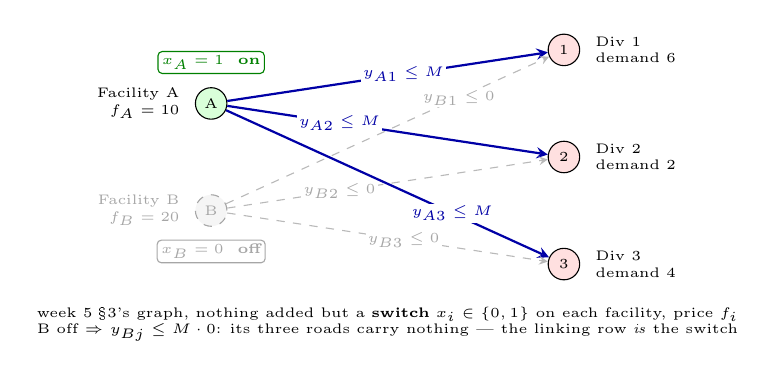
\begin{tikzpicture}[scale=0.8, font=\tiny, >=stealth,
    sw/.style={draw, rounded corners=1.5pt, inner sep=1.5pt, fill=white}]
  % facility A: switch on
  \node[circle, draw, fill=green!15, inner sep=1.4pt, minimum size=4mm] (sA) at (0,2.55) {A};
  \node[anchor=east, align=right] at (-0.35,2.55) {Facility A\\ $f_A = 10$};
  \node[sw, draw=green!50!black, text=green!50!black, font=\tiny\bfseries] at (0,3.2) {$x_A = 1$ \ on};
  % facility B: switch off --- node and roads fade
  \node[circle, draw, dashed, gray!70, fill=gray!8, text=gray!70, inner sep=1.4pt, minimum size=4mm] (sB) at (0,0.85) {B};
  \node[anchor=east, align=right, gray!70] at (-0.35,0.85) {Facility B\\ $f_B = 20$};
  \node[sw, draw=gray!70, text=gray!70, font=\tiny\bfseries] at (0,0.2) {$x_B = 0$ \ off};
  \foreach \j/\y/\dem in {1/3.4/6, 2/1.7/2, 3/0.0/4} {
    \node[circle, draw, fill=red!12, inner sep=1.4pt, minimum size=4mm] (d\j) at (5.6,\y) {$\j$};
    \node[anchor=west, align=left] at (5.95,\y) {Div \j\\ demand \dem};}
  \foreach \j in {1,2,3} { \draw[->, thick, blue!65!black] (sA) -- (d\j); }
  \foreach \j in {1,2,3} { \draw[->, dashed, gray!55] (sB) -- (d\j); }
  \foreach \j/\p in {1/0.55, 2/0.35, 3/0.7}
    \path (sA) -- node[pos=\p, fill=white, inner sep=0.8pt, text=blue!65!black] {$y_{A\j} \le M$} (d\j);
  \foreach \j/\p in {1/0.72, 2/0.35, 3/0.55}
    \path (sB) -- node[pos=\p, fill=white, inner sep=0.8pt, text=gray!70] {$y_{B\j} \le 0$} (d\j);
  \node[align=center] at (2.8,-0.95) {week 5 \S 3's graph, nothing added but a \textbf{switch} $x_i \in \{0,1\}$ on each facility, price $f_i$\\
    B off $\Rightarrow$ $y_{Bj} \le M \cdot 0$: its three roads carry nothing --- the linking row \emph{is} the switch};
\end{tikzpicture}
\end{center}
\begin{board}
\emph{how big is $M$?} \ $y_{ij} \le d_j$ always $\Rightarrow$ $M = d_j$, smallest valid. \
$M = \sum_j d_j$: also valid, but looser --- the LP bound sags with it (week 2: the \emph{smallest} valid $M$)
\vspace{3pt}

\textbf{1. fix $x$} $\Rightarrow$ transportation falls out: \emph{all the hardness is in the binaries}
\vspace{2pt}

\textbf{2. big-$M$ costs the guarantee:} $y_{ij} \le M x_i$ belongs to no incidence matrix $\Rightarrow$ week 5's MCNF
proposition is gone. \ (not TU $\ne$ the LP lies: only \emph{some} $b$ must go fractional. \S 2 checks)
\end{board}
\key{every guarantee in week 5's note is a property of $A$ --- so every one is a single modeling decision away from being lost.}

% ---------------------------------------------------------------- 2
\beat{2}{Deterministic LAP --- MCNF $+$ Facility Location}
\begin{board}
Remember week 5's conservation row (MCNF)? \ the flow is now called $y$ --- nothing else changes:
\[
  \textstyle\sum_{j} y_{ij} \;-\; \sum_{j} y_{ji} \;=\; b_i \quad (\forall i \in V)
  \qquad \text{outflow} - \text{inflow} = \text{net supply}
\]
\emph{what is $b_i$ at a node?} \ stock placed there, minus demand --- and two slacks so the row can always balance:
\[
  b_i \;=\; \underbrace{r_i}_{\text{decision}} \;-\; \underbrace{d_i}_{\text{data}} \;+\; q_i \;-\; s_i
\]
$r_i \ge 0$ = reserve held at $i$ (cost $h_i$/ton), \quad $q_i \ge 0$ = unmet demand (penalty $u_i$), \quad
$s_i \ge 0$ = surplus (penalty $o_i$; not transportation's supply)
\vspace{1pt}

two scalars of \emph{data}: \ $B$ = the stock budget (tons available to preposition), \quad $p$ = the most facilities we may open
\[
\begin{aligned}
  \min_{x,\,r,\,y,\,q,\,s}\quad
    & \textstyle\sum_{i \in V} f_i x_i + \sum_{i \in V} h_i r_i + \sum_{(i,j) \in E} c_{ij} y_{ij}
      + \sum_{i \in V} u_i q_i + \sum_{i \in V} o_i s_i \\
  \text{s.t.}\quad
    & \textstyle\sum_{j} y_{ij} - \sum_{j} y_{ji} = r_i - d_i + q_i - s_i && (\forall i \in V) && \text{[MCNF's conservation]} \\
    & \textstyle\sum_{i \in V} r_i \le B && && \text{[budget: a knapsack row]} \\
    & r_i \le B\, x_i && (\forall i \in V) && \text{[linking --- week 2]} \\
    & \textstyle\sum_{i \in V} x_i \le p && && \text{[at most $p$ facilities]} \\
    & y, r, s \ge 0, \quad 0 \le q_i \le d_i, \quad x_i \in \{0,1\}
\end{aligned}
\]
five costs: open ($f_i$), hold ($h_i$), ship ($c_{ij}$), unmet demand penalty ($u_i$), surplus maintenance cost ($o_i$). \ every constraint is old
\end{board}

\par\medskip\needspace{6\baselineskip}
{\bfseries Numerical example}\par\nobreak\vspace{1pt}
\begin{center}
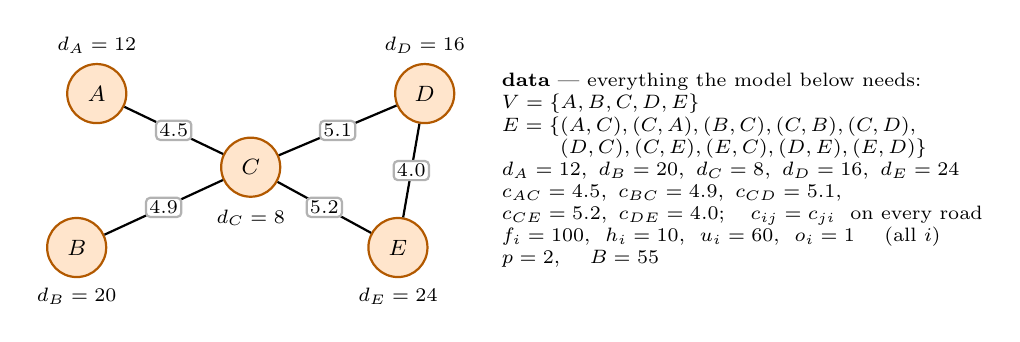
\begin{tikzpicture}[thick, font=\footnotesize, scale=0.85,
    site/.style={circle, draw=orange!70!black, fill=orange!20, minimum size=7.5mm},
    tt/.style={fill=white, draw=gray!60, rounded corners=1.5pt, inner sep=1.2pt, font=\scriptsize}]
  \node[site] (A) at (0, 1.6)    {$A$};
  \node[site] (B) at (-0.3, -0.7) {$B$};
  \node[site] (C) at (2.3, 0.5)   {$C$};
  \node[site] (D) at (4.9, 1.6)   {$D$};
  \node[site] (E) at (4.5, -0.7)  {$E$};
  \node[anchor=south, font=\scriptsize] at (0, 2.05)    {$d_A = 12$};
  \node[anchor=north, font=\scriptsize] at (-0.3, -1.15) {$d_B = 20$};
  \node[anchor=north, font=\scriptsize] at (2.3, 0.02)   {$d_C = 8$};
  \node[anchor=south, font=\scriptsize] at (4.9, 2.05)   {$d_D = 16$};
  \node[anchor=north, font=\scriptsize] at (4.5, -1.15)  {$d_E = 24$};
  \draw (A) -- node[tt] {$4.5$} (C);
  \draw (B) -- node[tt] {$4.9$} (C);
  \draw (C) -- node[tt] {$5.1$} (D);
  \draw (C) -- node[tt] {$5.2$} (E);
  \draw (D) -- node[tt] {$4.0$} (E);
  \node[anchor=west, align=left, font=\scriptsize] at (5.9, 0.45)
    {\textbf{data} --- everything the model below needs:\\
     $V = \{A, B, C, D, E\}$\\
     $E = \{(A,C), (C,A), (B,C), (C,B), (C,D),$\\
     $\phantom{E = \{} (D,C), (C,E), (E,C), (D,E), (E,D)\}$\\
     $d_A = 12, \ d_B = 20, \ d_C = 8, \ d_D = 16, \ d_E = 24$\\
     $c_{AC} = 4.5, \ c_{BC} = 4.9, \ c_{CD} = 5.1,$\\
     $c_{CE} = 5.2, \ c_{DE} = 4.0; \quad c_{ij} = c_{ji} \ $ on every road\\
     $f_i = 100$, \ $h_i = 10$, \ $u_i = 60$, \ $o_i = 1$ \quad (all $i$)\\
     $p = 2$, \quad $B = 55$};
\end{tikzpicture}
\end{center}
\begin{board}
that map, priced:
\[
\begin{aligned}
  \min\quad & \underbrace{100 \textstyle\sum_i x_i}_{\sum_{i \in V} f_i x_i}
    \;+\; \underbrace{10 \textstyle\sum_i r_i}_{\sum_{i \in V} h_i r_i}
    \;+\; \underbrace{60 \textstyle\sum_i q_i}_{\sum_{i \in V} u_i q_i}
    \;+\; \underbrace{\textstyle\sum_i s_i}_{\sum_{i \in V} o_i s_i} \\[10pt]
  & \quad + \underbrace{4.5\,(y_{AC} + y_{CA}) + 4.9\,(y_{BC} + y_{CB}) + 5.1\,(y_{CD} + y_{DC})
    + 5.2\,(y_{CE} + y_{EC}) + 4.0\,(y_{DE} + y_{ED})}_{\sum_{(i,j) \in E} c_{ij}\, y_{ij}}
\end{aligned}
\]
\vspace{-2pt}
\[
\begin{aligned}
  \text{s.t.}\quad
    & y_{AC} - y_{CA} = r_A - 12 + q_A - s_A && \text{[flow conservation (node $A$)]} \\
    & y_{BC} - y_{CB} = r_B - 20 + q_B - s_B && \text{[flow conservation (node $B$)]} \\
    & \textstyle (y_{CA}{+}y_{CB}{+}y_{CD}{+}y_{CE}) - (y_{AC}{+}y_{BC}{+}y_{DC}{+}y_{EC}) = r_C - 8 + q_C - s_C && \text{[flow conservation (node $C$)]} \\
    & (y_{DC} + y_{DE}) - (y_{CD} + y_{ED}) = r_D - 16 + q_D - s_D && \text{[flow conservation (node $D$)]} \\
    & (y_{EC} + y_{ED}) - (y_{CE} + y_{DE}) = r_E - 24 + q_E - s_E && \text{[flow conservation (node $E$)]} \\
    & \textstyle\sum_i r_i \le 55 && \text{[budget]} \\
    & r_A \le 55\, x_A && \text{[linking (node $A$)]} \\
    & r_B \le 55\, x_B && \text{[linking (node $B$)]} \\
    & r_C \le 55\, x_C && \text{[linking (node $C$)]} \\
    & r_D \le 55\, x_D && \text{[linking (node $D$)]} \\
    & r_E \le 55\, x_E && \text{[linking (node $E$)]} \\
    & \textstyle\sum_i x_i \le 2 && \text{[at most $p = 2$ facilities]} \\
    & y, r, s \ge 0, \quad 0 \le q_i \le d_i, \quad x_i \in \{0,1\}
\end{aligned}
\]
\end{board}
\par{\leavevmode\color{demoink}\small\textbf{demo}\quad\texttt{Deterministic-LAP-Demo.exe}}\par

\end{document}
